\documentclass[11pt]{article}
%%%%%%%%%%%%%%%%%%%%%%%%%%%%%%%%%%%%%%%%%

\usepackage{amscd}
\usepackage{amsmath}
\usepackage{amssymb}
\usepackage{amsthm}


\usepackage{epsfig}
\usepackage{verbatim}
\usepackage{graphicx}
\usepackage{amsthm}
\usepackage{hyperref}
\pagestyle{empty}
\usepackage{color}
\usepackage[left=0.85in,top=0.5in,right=0.85in,bottom=0.5in]{geometry} % Document margins
%\usepackage[all,dvips]{xy}


\begin{comment}  

This LaTeX document is a template to be used by Bates mathematics rising seniors to create a thesis proposal. 

As a guide, the document is already filled out to represent a fictitious proposal, and all you need to do is modify the entries below to represent your own proposal.

A PDF version of the fictitious proposal is available on the department's FAQ and Policies pages, at
http://abacus.bates.edu/acad/depts/math/faq.html
and
http://abacus.bates.edu/acad/depts/math/policies.html
respectively.

Once you have finished your proposal, export it to a PDF file. Give the file a USEFUL name, for example, RiemannThesisProposal.PDF. Email the PDF file to Clementine Brasier, the 
Academic Administrative Assistant for Hathorn Hall, at cbrasier\@bates.edu

This LaTex document was created Feb/Mar 2010 by Adriana Salerno and updated Feb 2012 by Meredith Greer

\end{comment}


%\setlength{\textheight}{8.5in} \setlength{\topmargin}{0.0in}
%\setlength{\headheight}{0.0in} \setlength{\headsep}{0.0in}
%\setlength{\leftmargin}{0.0in}
%\setlength{\oddsidemargin}{0.0in}
%%\setlength{\parindent}{1pc}
%\setlength{\textwidth}{6.5in}
%%\linespread{1.6}

\newtheorem{definition}{Definition}
\newtheorem{problem}{Problem}

\newtheorem{theorem}{Theorem}[section]
\newtheorem{lemma}[theorem]{Lemma}
\newtheorem{note}[theorem]{Note}
\newtheorem{corollary}[theorem]{Corollary}
\newtheorem{prop}[theorem]{Proposition}

%%%%%%%%%%%%%%%%%%%%%%%%%%%%%%%%%%%%%%%%%

\begin{document}
	\thispagestyle{empty}
	
	
	\centerline{\textbf{\Large{Binary Sentiment classification of Yelp reviews}}}
	
	\bigskip
	
	\textbf{Project Group Id:} 
	G5
	
	\bigskip
	
	\section{Introduction}
	Classification is one of the major tasks carried out in machine learning. Sentiment classification of text into categories such as positive and negative sentiment is one such task. Various machine learning approaches has been tried to solve this problem effectively in last two decades. We have taken up the task of sentiment classification of Yelp business reviews\cite{yelp} into positive and negative sentiments. Classification of reviews sentiments can help business understand user reviews about their service and help them in improving their service. In order to achieve this task, we explored four learning algorithms: Naive Bayes \cite{plv}, Support Vector Machines (SVM)\cite{plv}, Convolution Neural Network (CNN) \cite{kim} and Recurrent Neural Network (RNN) \cite{ydlb}. For Naive Bayes and SVM, we used unigram features as input. Word2vec \cite{w2v1} \cite{w2v2} features are used as input for CNN and RNN. In our experiments, on a dataset of 10K and 100K text reviews, we compared the performance of four different techniques. Out of fours methods, CNN gives us the best results with RNN a close second.
	
	\bigskip
	
	
	\section{Dataset and Features} 
		\subsection{Dataset}
		The original dataset described in the Yelp Dataset Challenge 9 \cite{yelp} has 4.1M reviews and 947K tips by 1M users for 144K businesses spread across four cities. In our experiments, we have considered set of 10K and 100K reviews randomly selected from set of 4.1M reviews. We considered two datasets, as for larger dataset it was difficult run non-linear SVM due to quadratic time complexity. For larger dataset, we considered Linear SVM during our experiment. The anonymized data is provided in JSON format for each review and each user profile. Each individual review data consists of anonymized IDs for the business, user and review, star rating  rounded to half-stars, review type and review text. We split the data into 80\% as training set and rest 20\% as testing set. Review with star rating less than or equal to 2.5 have been considered as negative and star rating greater than 2.5 as positive.   
	
		\subsection{Features}
			For each review text, we generated tokens using whitespace and converted all tokens to lower case. We have only considered tokens which were composed of only alphabets and had token length of at least three.
			\subsubsection{Unigram Features}
			Naive Bayes and SVM use unigram features as input to the algorithms. Initially, we created a vocabulary using tf-idf score for each token and selecting top 5000 tokens based on the scores. Then, we created bag of words feature vector using the vocabulary for each review where presence of each word was considered as discussion in paper \cite{plv}. Bag of words feature vectors we used to train Naive Bayes classifier. Both linear and non-linear SVM were given tf-idf scores matrix of reviews for training.
			
			\subsubsection{Word2Vec Features}  
			Word2vec is a method proposed in paper \cite{w2v1} and improved in \cite{w2v2} for continuous vector representations of words obtained from an unsupervised neural language model using skip-grams or continuous bag of words models. In our experiments, two word2vec models were considered as done in \cite{kim}:
			\begin{enumerate}
				\item \textbf{Random model:} Baseline model where word vector are randomly initialized and then modified during training. It is also used as a baseline.
				\item \textbf{Non-static model:} Model trained on our review data using skip-grams to get word vector representation.
			\end{enumerate}
		
	\section{Methods}
		\subsection{Naive Bayes}
		Naive Bayes is a probabilistic classifier which assigns document d to a class $c \in C$ , which has maximum posterior probability given the document. In our experiment, given a document vector $d=(x_1,x_2,...,x_n)$, where n is the size of vocabulary, we want to label d to class with $\max{P(c|x_1,...,x_n)}$, the probability of a possible class. Using Bayes rule, 
			\[
				P(c|x_1,...,x_n) = P(c) \times P(x_1,...,x_n | c)
			\]  
		where $P(c)$  is prior probability and $P(x_1,...,x_n | c)$ is the likelihood of the document. We have only two classes, positive and negative sentiment for our task.
		
		\subsection{Support Vector Machines (SVM)}
		In contrast to Naive Bayes, SVMs are large margin classifiers rather than probabilistic classifier. It tries to find a hyperplane that separates the document vectors in one class from those in other class for which margin is as large as possible. Given a training data $(X_i, Y_i)$ for $i=1,2,..m$, where $X_i$ is feature vector which represents a document d and $Y_i \in \{-1, 1\}$, SVM tries to learn a classifier f(x) such that $Y_i \times f(X_i) \geq 1$. The support vectors are $X_i$ on the boundary for which $Y_i \times f(X_i) = 1$.
		
		\subsection{Convolution Neural Network (CNN)}
		Convolution neural networks (CNN) use layers with convolving filters that are applied to local features \cite{lecun}. CNN was originally invented for computer vision but it has been effective in various NLP applications. In our experiment, we used CNN model architecture suggested by Kim \cite{kim} with few changes. Model suggested by Kim \cite{kim} had total four layers: two-channel input word2vec layers, convolution layers with multiple filters, max-over-time pooling layer and fully connected output layer with dropout and softmax output. Our model shown in figure \ref{fig:cnn} has only one channel input layer compared to Kim's model. In addition, we have one hidden layer, a fully connected layer with ReLu activation, before the sigmoid output layer. 
		
		Each review is considered as a single training data, which is represented by $R^nk$ matrix where each row vector represents a single token from the review with k features. We have done padding of sentences to make each sentence equal to n where n is either maximum sentence length in data or 400 whichever in minimum. Convolution layer has multiple filters with three different sizes 3,4 and 5 as used by Kim \cite{kim}. Max-over-time layers takes maximum of all values from a feature layers created by one filter. The idea is to capture the most important feature for each feature map. This pooling scheme also helps in dealing with variable sentence lengths. 
		
		Features obtained after max-over-time pooling, is then applied to a fully connected dense network with ReLu activation. Final layer is a fully connected layer with one output neuron and sigmoid activation. For regularization, we have used dropout on penultimate layer. It prevents co-adaptation of hidden units by a randomly dropping out a proportion of hidden units during forward backpropagation. We have used dropout rates of 0.5 and 0.8. 
		
		\begin{figure}
			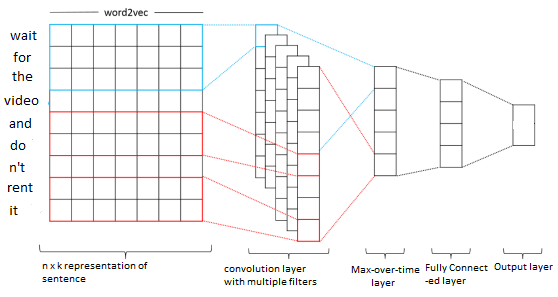
\includegraphics[width=\linewidth]{CNN.png}
			\caption{CNN Model architecture $(Image Courtesy:Kim \cite{kim})$. }
			\label{fig:cnn}
		\end{figure}
		\subsection{Recurrent Neural Network (RNN)}
		
		RNN is a class of artificial neural network with sequential data where each neuron or unit can use internal memory to maintain information about the previous input. This helps the neural network to form a connection between unit to a directed cycle and allows the network to gain deeper understanding of the statement. A RNN has loops in them that allow information to be carried across neurons while reading in input.\\
		
		As discussed in the paper \cite{ydlb} we tried the discriminative approach by ingesting and outputting one symbol at a time in the RNN unit, where the last step output is also a new time step's input. In our model the input to text classification system are a document x=$\{x_1,x_2..,x_T\}$, where T is its length in words and we predict a label $y \in Y$. Discriminative models are trained to distinguish the correct label among the possible choices.
		
		Our model uses LSTM $(Long-Short Memory Network)$ with peephole connections to encode a document and build a classifier on top of encoder by using the average of LSTM hidden representation as the document representation. So given an input word embedding $x_t$, we compute its hidden representation $h_t \in \mathbb{R}^E$ with LSTM as shown in Figure \ref{fig:rnn} $($Haven't shown the mathematical formula to show the computation, please refer the \cite{ydlb} for the formula$)$.\\
		
		In implementation we have mapped each yelp review into a real vector domain also known as word embedding or word2vec. In this the words are encoded as real valued vectors in a high dimensional space, where the similarity between words translates to closeness in vector space. As in the paper our first layer is the embedded layer that uses 300 length vector to represent each word. The next layer is the LSTM layer with 100 memory units$($small neurons$)$. Also since this is a classification problem we have used a sigmoid function and a dense output layer with a single neuron. We have used AdaGrad algorithm to train our model. A considerable batch size of 64 reviews is used to distribute the weight updates. To avoid over-fitting in our RNN we have applied dropout layer between the Embedding-LSTM layer and the LSTM-DenseOutput layers. As in CNN we have used the droupout rates of 0.5 and 0.8.
		
		
		\begin{figure}
			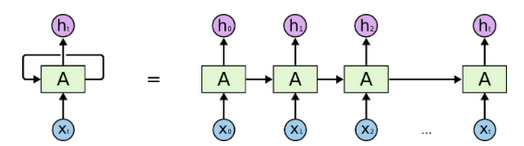
\includegraphics[width=\linewidth]{Rnn.png}
			\caption{An unrolled RNN$(Image Courtesy:Cameron Godbout)$. }
			\label{fig:rnn}
		\end{figure}
	
	\section{Experiments and Results}
		\subsection{Naive Bayes and SVM}
		In order to extract the vocabulary we have used tf-idf scores and then selected top 5000 words. We trained the Naive Bayes with unigram feature vectors representing one review from the dataset. In a feature vector of a review, 1 is used if the given word from vocabulary is present in that review and 0 if word is not present. We trained naive bayes for 10K and 100k dataset.
		
		As non-linear SVM classification is quadratic time algorithm, we used linear SVM for larger 100K dataset. Tf-idf score matrix with vocabulary size 5000 were used a an input to SVM classifier. Performance of linear SVM reduced drastically compared to non-linear SVM even after significant increase in training data. It shows the non-linear relation of reviews with sentiments.
		
		We used Naive bayes as the baseline method and given that its performance is worst among all the techniques is no surprise. However, we were expecting better performance from SVM which goes to show that data is not linearly separable.
		\begin{table}
		\caption{Model Accuracy Results} 
		\begin{center}
			\begin{tabular}{|c|c|c|}
				
				\hline
				Dataset & Naive Bayes & SVM/Linear SVM \\
				\hline
				\hline
				10K & 75.4\%  & 76.0\% \\
				\hline
				100K & 76.13\% & 64.78\% \\
				\hline
			\end{tabular}
			 
		\end{center}
		\end{table}
		\subsection{CNN and RNN}
		As mentioned above, we had considered two type input word2vec model. First model was randomly initialized vector with 300 features or dimension which was then modified during training. Non-static model was again a 300 dimension model which was obtained after training on 100K unlabeled reviews using skip-grams. 
		
		For CNN, we have 10 filters each of height 3, 4 and 5 as filter with height more than 5 or more often produce noise in text classification. Thus, after max-over-pooling, we have a 30 x 1 feature map. Number of neurons in fourth fully connected layer is 30. We could have experimented with more hyper-parameters, but due to very long running time it was not possible in our time frame.
		
		Similar to CNN, we used both type of word2vec for training the models with 300 dimensions each. We have used 100 LSTM layers along with dropout layer and a fully connected output layer with sigmoid activation. As observed by Kim \cite{kim}, non-static word2vec model tends to preform slightly better than random models. While comparing CNN and RNN, CNN performs slightly better also observed in work \cite{ydlb}. 
		
			\begin{table}
				\caption{Model Accuracy Results} 
				\begin{center}
					\begin{tabular}{|c|c|c|c|c|}
						
						\hline
						Dataset & CNN-rand & CNN-non-static & RNN-rand & RNN-non-static \\
						\hline
						\hline
						10K & 88.01\%  & 88.25\% &  86.7\% & 86.9\%\\
						\hline
						100K & 90.88\% & 91.21\% & 90.16 & 91.02\% \\
						\hline
					\end{tabular}
					
				\end{center}
			\end{table}
		    	
	\section{Discussion and future work}
	In our future work, we could try using pre-trained word2vec vectors that were trained on 100 billion words from Google News. The vectors have dimensionality of 300 and were trained using the continuous bag-of-words architecture \cite{miko}. In addition, we can explore generative RNN models as we have only considered discriminative models. Also we can use Gated Recurrent Units(GRU) along with LSTM and compare which one performs better. We should also try to train on much larger dataset to more fine tune the models.					
	
	\begin{thebibliography}{99}
		% NOTE: change the "9" above to "99" if you have MORE THAN 10 references.
		
		\bibitem{yelp} Yelp Dataset Challenge \url{https://www.yelp.com/dataset_challenge}
		\bibitem{plv} Bo Pang, Lillian Lee and Shivakumar Vaithyanathan. \textit{Thumbs up? Sentiment Classification using Machine Learning
			Techniques}, In EMNLP, 2002.   
		
		\bibitem{kim} Yoon Kim. \textit{Convolutional Neural Networks for Sentence Classification}, In EMNLP, 2014.
		
		\bibitem{ydlb} Dani Yogatama, Chris Dyer, Wang Ling and Phil Blunsom. \textit{Generative and Discriminative Text Classification
			with Recurrent Neural Networks}, arXiv preprint arXiv:1703.01898, 2017
		\bibitem{w2v1} Tomas Mikolov, Ilya Sutskever, Kai Chen, Greg Corrado and Jeffrey Dean. \textit{Distributed Representations of Words and Phrases and their Compositionality}, In NIPS, 2013
		\bibitem{w2v2} Tomas Mikolov,, Kai Chen, Greg Corrado, and Jeffrey Dean. \textit{Efficient estimation of word representations in vector space}, In ICLR 2013
			
		\bibitem{lecun} Y. LeCun, L. Bottou, Y. Bengio, P. Haffner. \textit{Gradient-based learning applied to document recognition}
		In Proceedings of the IEEE, 86(11):2278–2324, November, 1998 
		
		\bibitem{miko} Q. Le, T. Mikolov. \textit{Distributed Representations of Sentences and Documents}, In Proceedings of ICML 2014
		
	\end{thebibliography}
	
	\newpage
	\appendix
	
	\section{Source Code:} Source has been provided as separate attachment while submitting on blackboard. Code is compliled in Python 3.5. In order to run, run the process.py file in commandline with following option arguments.
	\begin{enumerate}
		\item algo: 1(Naive Bayes), 2(SVM), 3(CNN), 4(RNN)
		\item data\_file: 2(10K Dataset), 3(100K dataset)
		\item reloadData: False,True(True for first time run)
		\item model\_type: rand, non-static(only for CNN and RNN)
	\end{enumerate}
	
	\section{Statement of contribution:}
		\subsection{Authors} Aditya Priyadarshi, Yogesh Gupta, Aditya Sridhar  and Shubham Sharma
		
		\subsection{Contributions:}
	 Initially, all four members of the team discussed together in selecting a project topic and then understanding the data. All of us studied the related work done in order to solve the sentiment classification task. Then, each of us select one algorithm and then delved deeper into understanding the technique and applying to our data.
	 
	 Shubham worked on applying Naive Bayes algorithm to our dataset. Aditya Sridhar worked with SVM algorithm. Yogesh Gupta was involved in understanding how recurrent neural network is applied to our task and then implemented the model. Aditya Priyadarshi worked on convolution neural network model where he tried different hyper-parameters to get the best results. Aditya Priyadarshi and Yogesh also worked together in understanding word2vec model and how to apply to our task.
	 
	 All of us equally contributed towards writing the final report as each of us worked on different learning algorithms. 
		
	%%%%%%%%%%%%%%%%%%%%%%%%%%%%%%%%%%%%%%%%%
	
	
	
	
	
	
\end{document} 
